\documentclass[header]{subfiles}
\begin{document}

\providecommand{\rootdir}{.}

\chapter{Coherence}
\label{chapter:Coherence}


% \green{Explicar qué es coherencia.}
% \medskip

In simple worlds, \emph{coherence} is a state or measure of some \emph{pieces}
fitting together into a whole. Coherence can be applied to almost any aspect of
the universe. Stable orbits require coherence between the observed laws of physics
and universal constants, the speeds and masses of the bodies in the system.
A healthy society asks for coherence between the people and their roles within
the system. An organism requires coherence between its organs in order to operate;
its interactions with the environment must be coherent with its necessities and
surrounding conditions. The notion of coherence is very powerful because of its
generality. Based on a proper logic, coherence can be used to judge about systems
and to test different situations or proposals.

\begin{displayquote}
The consistency or \emph{coherence} within a logical or mathematical
system, means that $p$ and $\neg p$ must not be derivable from the
basic assumptions in accordance with the observance of the syntactical
rules \cite{Daya60}.
\end{displayquote}


\section{Coherence theory}
\label{sec:CoherenceTheory}

\begin{displayquote}
Coherence theory is a psychologically motivated motivational cognitive theory with
foundations in philosophy that approaches problems in terms of the satisfaction
of multiple constraints within networks of highly interconnected elements
\cite[p.~19]{UAB-Thesis}.
\end{displayquote}

Thagard, in his work \cite{Thagard89}, shows how \emph{explanatory coherence}
can be used to test hypothesis against propositions for proving scientific theories
and reasoning about many other situation. He says that a hypothesis coheres
with given propositions if it explains, is explained, offers analogous explanation or
participates in other explanations. The propositions that stand for observations
have a degree of acceptability. Propositions are incoherent if they contradict
each other.

Another interesting usage, given by Thagard, using his \emph{explanatory coherence}
theory for \emph{Adversarial Problem Solving} (APS).
APS consists in understanding of opponent's strategy and anticipation of his actions
with the purpose of successful counteraction and ultimate victory.
These problems are competition ones: it could be war or business strategy,
different games, and any other areas, that involve gaining the upper hand
on adversaries. Thagard states that the judgments, based on the coherence theory,
can be important for inferring the plans of the opponent and deceiving him
\cite{ThagardAPS92}.

\medskip

Later Thagard published that coherence can be understood in terms of maximal satisfaction
of multiple constraints and in this form it can be used to solve problems in
diverse areas, such as logic, mathematics, law, ethics, rationality, etc \cite{ThagVerb98}.

In his theory, the coherence problem is about partitioning a graph of
\emph{information pieces}, interconnected by positive or negative weighted
constraints, that enhance or diminish partition's coherence.
The coherence-maximizing partition is the one that has maximum number of constraints
satisfied.

An example of partitioning by Thagard's method is given in figure \ref{fig:UAB-partition}.
The information graph $\mathcal{V}$ consists of
classes $C_1,\dots,C_4$, also there are three possibilities for
class $C_1$ placement and two for class $C_4$. A relation is
\begin{itemize}[leftmargin=3cm]
  \item[\red{\emph{inconsistent}}], if two classes intersect in time;
  \item[\orange{\emph{same class}}], if two classes differ only by time;
  \item[\green{\emph{consistent}}], otherwise.
\end{itemize}

\noindent
The coherence of the partition $\mathcal{A},\mathcal{V}\backslash\mathcal{A}$
          is calculated as
\medskip

$   \dfrac{ \text{\green{\emph{consistent}} relations in } \mathcal{A}
          + \text{\red{\emph{inconsistent}} relations between }
                  \mathcal{A} \text{ and } \mathcal{V}\backslash\mathcal{A}}
          {\text{total relations in } \mathcal{V}}$.
\medskip

\noindent
It's value is $\frac{|1| \cdot 3 + |-1| \cdot 5}{17} \approx 0.47$.


\begin{figure}[h]
  \centering
  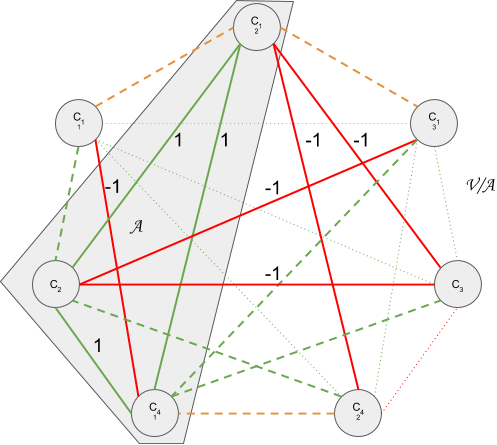
\includegraphics[width=0.5\textwidth]{\rootdir/img/UAB-splitting.png} % scale=0.5
  % \captionsetup{singlelinecheck=off}
  \caption[Information graph partitioning example]
          {Example: information graph partitioning, proposed by Thagard
           \cite{UAB-Thesis, ThagVerb98}. }
  \label{fig:UAB-partition}
\end{figure}



\section{Coherence and Contexts}
%%%%%%%%%%%%%%%%%%%%%%%%%%%%%%%%%%%%%%%%%%%%%%%%%%%%%%%%%%%%%%%%%%%%%%%%%%%%%%%%
\label{sec:Coherence-Cxts}

In PHD thesis \cite{UAB-Thesis}, the author establishes concrete
\emph{coherence functions}, based on the properties, proposed by Thagard for
such functions. The author chooses \emph{g-BDI} agent architecture ---
a \emph{multi-context} system, where the contexts are: \emph{beliefs},
\emph{desires} and \emph{intentions}. Each context has its \emph{internal rules}
for computing context's logics and there are \emph{bridge rules} that allow to
import contexts' results into other contexts. It should be noted, that \emph{g-BDI}
architecture uses \emph{fuzzy logics}.

The \emph{information graph} is obtained by joining contexts' graphs with the
help of \emph{bridge rules}  \cite[p.62]{UAB-Thesis}.

\bigskip

% \green{Explicar cómo se puede usar para resolver el problema de Scheduling}
% \medskip

\noindent
In this thesis a different approach is taken.
% The initial information graph,
% composed of \emph{classes propositions}, is passed to a \emph{splitting} context,
% that generates all posiible \emph{acceptable} (by the splitting context) sub-graphs,
% called \emph{candidates} (as it will be shown in \emph{Beliefs} context).
A set of class propositions or a \emph{candidate} forms initial information graph,
that is propagated through the \emph{filtering contexts} in the established
order. At each context it gets assessed
(using context-specific knowledge and relations)
and the result is compared against context-specific threshold.
If passing threshold test,
the candidate is sent to the next context, otherwise it is marked as failed
(providing a reason) and is propagated no further. In both cases the coherence
value and some context defined \emph{details} are guarded alongside the candidate.

Thus a context in this thesis serves as \emph{candidates} filter. This approach
\textbf{allows to avoid}:
\begin{enumerate}
  \item Usage of \emph{bridge rules}. It permits more flexibility for
    the \emph{internal rules}. Changes in contexts' logic do not affect the way
    the results are combined, even if the changes are incompatible.
  \item Huge graph partitioning. Such graph would have to unite \emph{all the
    candidates} and every context's internal knowledge. Then the entire graph
    needs to be stored, until the best partition is found.

    In the proposed approach, both \emph{candidates generation} and
    \emph{filtering} can be done sequentially and
    lazily\footnote{Instead of storing value(s), \emph{lazy} evaluation
                    strategy stores \emph{how to create} them.
                    Evaluation is performed only when a value is needed.},
    thereby reducing memory usage.

\end{enumerate}

\end{document}
